\chapter{Data and measurement}\label{ch:data}

\section{Sources}
All data come from public archives, downloaded and parsed with scripts so that every step can be repeated
(Appendix~\ref{app:data}).
\begin{table}[h]\centering\small
\caption{Data sources}\label{tab:sources}
\begin{tabularx}{\textwidth}{>{\raggedright\arraybackslash}p{4.3cm}L>{\raggedright\arraybackslash}p{2.9cm}}
\toprule
Source & Content & Coverage \\
\midrule
NSE combined open interest files & MWPL, open interest, futures-equivalent open interest (from Oct 2025), next-day status & Feb 2010 to Oct 2026 \\
NSE securities-in-ban lists & Official ban list & Feb 2010 to Oct 2026 \\
NSE F\&O and cash bhavcopies, delivery files & Prices, traded value and quantity, contracts, open interest, delivery & 2015 to Oct 2026 \\
NSE corporate actions & Dividends, splits, bonuses and other events with ex-dates & 2014 to 2026 \\
NSE announcements, results filings, board meetings & First dissemination time of quarterly results & 2014 to 2026 \\
NSE SLB bhavcopies & Daily securities-lending trades and fees & 2015 to Oct 2026 \\
AMFI & Half-yearly average market capitalisation lists; monthly arbitrage-fund flows and assets & 2017 to 2026; Apr 2018 to Sep 2026 \\
OECD via FRED & Three-month interbank rate (monthly) & 2011 to 2026 \\
\bottomrule
\end{tabularx}
\end{table}

\section{Checks}
Of the 11,764 daily ``no fresh positions'' flags, 11,753 (99.9\%) match the next day's official ban list; utilisation
exceeded 95\% on the day before 99.4\% of ban spells began and was at or below 80\% on the last day of 99.7\%. On three days
the official list is missing at the exchange; those lists are imputed from the previous day's flags and continuing spells
and flagged. The set of stocks in the open interest files matches the stock futures in the F\&O bhavcopy, and an
independent daily membership file for 2016 to 2025 agrees on every stock-day. The futures volume-weighted average price
lies inside the day's range for 99.8\% of contracts after recovering lot sizes in the older files. Results announcements
are dated from the exchange's first dissemination time; the results filings alone often carry later re-filing times and
current rather than historical symbols, so announcements, board meetings and the history of each security's identifier
are combined, which covers 98\% to 100\% of F\&O stock-quarters.

\section{Bans}
\begin{table}[h]\centering\small
\caption{F\&O bans by year, 2015 to 2026}\label{tab:bans}
{\footnotesize\setlength{\tabcolsep}{4pt}\begin{tabular}{lrrrrrr}
\toprule
Year & \shortstack[r]{F\&O stocks\\(avg per day)} & \shortstack[r]{Stocks\\banned} & \shortstack[r]{Ban\\spells} & \shortstack[r]{Ban\\stock-days} & \shortstack[r]{Median spell\\(days)} & \shortstack[r]{Longest spell\\(days)} \\
\midrule
2015 & 154 & 16 & 69 & 367 & 4 & 21 \\
2016 & 172 & 27 & 136 & 645 & 4 & 17 \\
2017 & 200 & 43 & 287 & 1586 & 5 & 24 \\
2018 & 206 & 38 & 162 & 810 & 4 & 31 \\
2019 & 176 & 23 & 86 & 508 & 4 & 17 \\
2020 & 140 & 40 & 178 & 756 & 3 & 13 \\
2021 & 163 & 26 & 162 & 789 & 4 & 16 \\
2022 & 196 & 23 & 100 & 457 & 4 & 13 \\
2023 & 187 & 41 & 193 & 942 & 4 & 17 \\
2024 & 185 & 49 & 289 & 1656 & 5 & 22 \\
2025 & 216 & 37 & 94 & 556 & 5 & 15 \\
2026$^{a}$ & 209 & 10 & 33 & 342 & 10 & 29 \\
\midrule
2015 to 2026 & 183 & 141 & 1789 & 9414 & 4 & 31 \\
\bottomrule
\end{tabular}
}

\vspace{3pt}{\footnotesize January to 27 October 2026. Spells are counted in the year they start.}
\end{table}
Over 2015 to 2026 there were 1,788 ban spells covering 9,416 stock-days and 141 stocks. Bans are concentrated: the most
frequently banned stock had 76 spells. Before October 2025 the median spell lasted four trading days; the 44 spells since
then have a median of nine. On 1 October 2025 the new formula lowered the MWPL of all 208 F\&O stocks, to a median of 73\%
of the old value (Figure~\ref{fig:mwpl}).

\begin{figure}[h]\centering
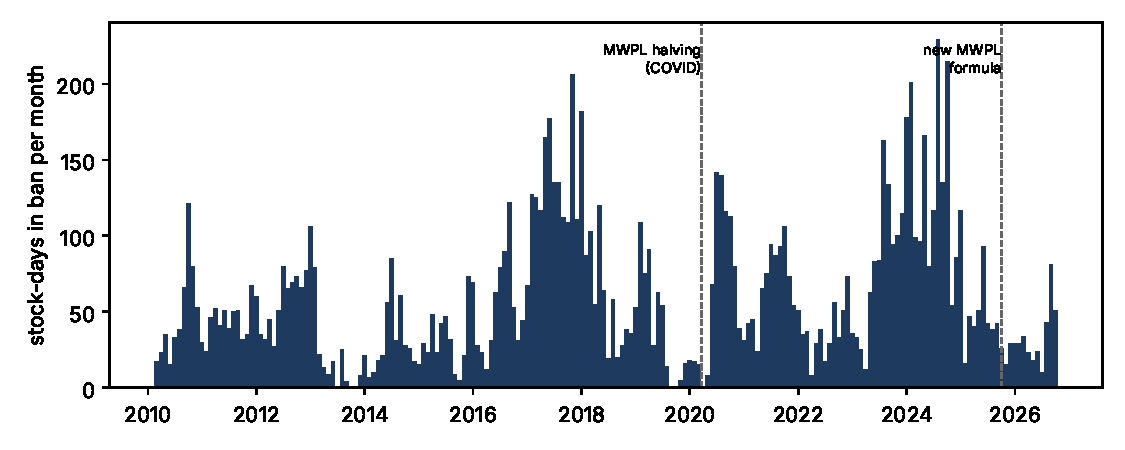
\includegraphics[width=0.9\textwidth]{ban_days_per_month.pdf}
\caption{Stock-days in the F\&O ban per month, 2010 to 2026.}\label{fig:bandays}
\end{figure}
\begin{figure}[h]\centering
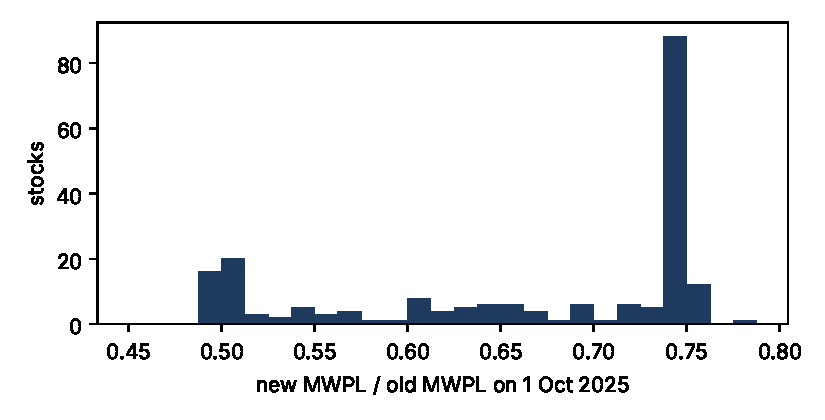
\includegraphics[width=0.6\textwidth]{mwpl_ratio_oct2025.pdf}
\caption{Ratio of the new to the old MWPL on 1 October 2025, all F\&O stocks.}\label{fig:mwpl}
\end{figure}

\section{The basis}
For each stock and day, the basis is computed from the volume-weighted average prices of the future and of the stock, net
of dividends going ex before expiry and of carry at the three-month interbank rate:
\[ m_{it}=\ln\bar F_{it}-\ln\big(\bar S_{it}-\mathrm{PV}_{it}(D)\big)-r_t\tau_{it}. \]
The near-month contract is used, switching to the next month when three or fewer trading days remain; at least five
contracts must trade; contracts with a dividend or other corporate event in their life and the first 20 trading days after
a stock enters the F\&O segment are excluded; the basis is winsorised at 1\% and 99\% within each year. The resulting sample
has 486,040 stock-days for 371 stocks, 8,851 of them in a ban. On the clean sample the median basis is $+1.2$\bp, and the
10th and 90th percentiles are $-33.0$ and $+26.2$\bp; the lower tail is wider than the upper. The basis shrinks toward
expiry. A relative implied repo rate (the stock's implied financing rate minus the day's cross-sectional median) and a
basis built from closing prices are used as checks.

\section{Other outcomes}
\begin{itemize}
\item \emph{Trading:} futures contracts traded (near and next month), the change in open interest in contracts, the ratio
$R=(\Delta OI+V)/V$, cash volume and the delivery share.
\item \emph{Earnings drift:} the buy-and-hold return over days $+2$ to $+64$ after a results announcement minus that of the
stock's size-decile portfolio; the surprise is the abnormal return over days $-1$ to $+1$; bad (good) news is the bottom
(top) tercile within each quarter. Returns are adjusted for splits, bonuses and dividends (the exchange's previous-close
field is not), and events with a price below Rs 5 are excluded.
\item \emph{Price delay:} the share of a stock's weekly return variation explained by lagged market returns (Hou and
Moskowitz, 2005), by calendar year.
\end{itemize}

\section{A constraint index for all stocks}\label{sec:index}
To measure how hard arbitrage is in each stock without using the outcomes or the treatments, I build a quarterly index for
all NSE stocks (80,042 stock-quarters, 3,310 stocks, 2015 to 2026) from five frictions: no short channel (not in the F\&O
segment), SLB scarcity (share of days without any SLB trade), the Corwin and Schultz (2012) spread, Amihud (2002)
illiquidity and idiosyncratic volatility. Each is standardised within the quarter, and the index is their first
principal component, which explains 53\% of their variance; all five load positively (0.37 to 0.49) and the loadings are
stable from year to year. The index is persistent (quarter-to-quarter rank correlation 0.90).

\begin{table}[h]\centering\small
\caption{Validation of the constraint index (frictions measured before outcomes)}\label{tab:index}
\begin{tabular}{lccc}
\toprule
Outcome & Per s.d.\ (s.e.) & Size-controlled & Obs. \\
\midrule
Price delay, next year (year FE) & $+0.058$ (0.003) & $+0.036$ (0.004) & 15,790 \\
Price delay, next year (stock and year FE) & $+0.032$ (0.005) & $+0.028$ (0.006) & 15,790 \\
Absolute drift after announcements & $+0.023$ (0.001) & $+0.015$ (0.001) & 69,673 \\
Drift after bad news & $-0.008$ (0.001) & $-0.001$ (0.002) & 23,219 \\
Drift after good news & $+0.001$ (0.001) & $+0.001$ (0.002) & 23,095 \\
\bottomrule
\end{tabular}

\vspace{2pt}\parbox{0.92\textwidth}{\footnotesize FE: fixed effects. Size control: log market capitalisation for price delay (15,227 stock-years with a market capitalisation); market-capitalisation decile fixed effects for drift.}
\end{table}
More constrained stocks respond more slowly to market news, also within a stock over time and after controlling for size,
and drift more after announcements in either direction (Table~\ref{tab:index}). Without a size control, drift after bad
news, but not good news, is stronger for more constrained stocks; with size-decile fixed effects this asymmetry disappears,
so it reflects the smaller size of constrained stocks rather than the short-sale constraint. These are associations. Within F\&O stocks, the short-channel component does not vary and SLB activity
appears to reflect demand to borrow rather than ease of borrowing, so for the futures-cash band of F\&O stocks I use a
separate F\&O index that adds utilisation of the position limit (Chapter~\ref{ch:band}).
